\documentclass[10pt]{article}
\usepackage[margin=1in]{geometry}
\usepackage[T1]{fontenc}
\usepackage{times}
\usepackage{amsmath,amssymb,amsthm}
\usepackage{booktabs,tabularx,array}
\usepackage{graphicx}
\usepackage{xcolor}
\usepackage[hidelinks]{hyperref}
\usepackage{enumitem}
\usepackage[font=small,labelfont=bf]{caption}
\usepackage{subcaption}
\setlist{nosep,leftmargin=1.3em,topsep=2pt}
\setlength{\parskip}{3pt}
\newtheorem{proposition}{Proposition}
% Generated by experiments/analyze.py. Do not edit.
\newcommand{\nScenarios}{880}
\newcommand{\nInvariantScenarios}{848}
\newcommand{\nScopeScenarios}{32}
\newcommand{\nTwinClusters}{424}
\newcommand{\nFamilies}{27}
\newcommand{\nSeedsFamily}{16}
\newcommand{\nArms}{27}
\newcommand{\nEpisodes}{23,760}
\newcommand{\nProposals}{2,092}
\newcommand{\nCatOne}{184}
\newcommand{\nCatTwo}{112}
\newcommand{\nCatThree}{456}
\newcommand{\nCatFour}{128}
\newcommand{\verifierDisagreements}{0}
\newcommand{\nLegit}{312}
\newcommand{\givrCzero}{59.0\%}
\newcommand{\givrCzeroCI}{[53.2, 64.4]}
\newcommand{\uarCzero}{90.1\%}
\newcommand{\uarCzeroCI}{[87.2, 92.6]}
\newcommand{\frrCzero}{0.0\%}
\newcommand{\frrCzeroCI}{[0.0, 0.0]}
\newcommand{\frrCzeroUpper}{0.8\%}
\newcommand{\ltcrCzero}{92.3\%}
\newcommand{\ltcrCzeroCI}{[86.8, 96.9]}
\newcommand{\sevCzero}{\$2,448}
\newcommand{\scopeCzero}{32}
\newcommand{\unsafeNCzero}{544}
\newcommand{\commitNCzero}{544}
\newcommand{\gapCzero}{0.0\%}
\newcommand{\givrKCzero}{500}
\newcommand{\givrCone}{38.2\%}
\newcommand{\givrConeCI}{[34.3, 42.0]}
\newcommand{\uarCone}{57.3\%}
\newcommand{\uarConeCI}{[54.1, 60.5]}
\newcommand{\frrCone}{5.2\%}
\newcommand{\frrConeCI}{[3.9, 6.6]}
\newcommand{\ltcrCone}{74.4\%}
\newcommand{\ltcrConeCI}{[68.4, 80.3]}
\newcommand{\sevCone}{\$2,484}
\newcommand{\scopeCone}{32}
\newcommand{\unsafeNCone}{346}
\newcommand{\commitNCone}{346}
\newcommand{\gapCone}{0.0\%}
\newcommand{\givrKCone}{324}
\newcommand{\givrCtwo}{29.2\%}
\newcommand{\givrCtwoCI}{[25.3, 33.0]}
\newcommand{\uarCtwo}{44.7\%}
\newcommand{\uarCtwoCI}{[41.2, 48.1]}
\newcommand{\frrCtwo}{3.6\%}
\newcommand{\frrCtwoCI}{[2.4, 4.8]}
\newcommand{\ltcrCtwo}{77.6\%}
\newcommand{\ltcrCtwoCI}{[71.5, 83.7]}
\newcommand{\sevCtwo}{\$2,408}
\newcommand{\scopeCtwo}{32}
\newcommand{\unsafeNCtwo}{270}
\newcommand{\commitNCtwo}{270}
\newcommand{\gapCtwo}{0.0\%}
\newcommand{\givrKCtwo}{248}
\newcommand{\givrCthreeKone}{50.7\%}
\newcommand{\givrCthreeKoneCI}{[44.6, 56.3]}
\newcommand{\uarCthreeKone}{74.8\%}
\newcommand{\uarCthreeKoneCI}{[70.2, 78.7]}
\newcommand{\frrCthreeKone}{1.1\%}
\newcommand{\frrCthreeKoneCI}{[0.5, 1.8]}
\newcommand{\ltcrCthreeKone}{89.7\%}
\newcommand{\ltcrCthreeKoneCI}{[83.9, 94.5]}
\newcommand{\sevCthreeKone}{\$2,150}
\newcommand{\scopeCthreeKone}{32}
\newcommand{\unsafeNCthreeKone}{452}
\newcommand{\commitNCthreeKone}{452}
\newcommand{\gapCthreeKone}{0.0\%}
\newcommand{\givrKCthreeKone}{430}
\newcommand{\givrCfour}{0.0\%}
\newcommand{\givrCfourCI}{[0.0, 0.0]}
\newcommand{\givrCfourUpper}{0.8\%}
\newcommand{\uarCfour}{0.0\%}
\newcommand{\uarCfourCI}{[0.0, 0.0]}
\newcommand{\uarCfourUpper}{0.8\%}
\newcommand{\frrCfour}{0.0\%}
\newcommand{\frrCfourCI}{[0.0, 0.0]}
\newcommand{\frrCfourUpper}{0.8\%}
\newcommand{\ltcrCfour}{92.3\%}
\newcommand{\ltcrCfourCI}{[86.8, 96.9]}
\newcommand{\sevCfour}{\$0}
\newcommand{\scopeCfour}{32}
\newcommand{\unsafeNCfour}{0}
\newcommand{\commitNCfour}{0}
\newcommand{\gapCfour}{0.0\%}
\newcommand{\givrKCfour}{0}
\newcommand{\givrCfive}{0.0\%}
\newcommand{\givrCfiveCI}{[0.0, 0.0]}
\newcommand{\givrCfiveUpper}{0.8\%}
\newcommand{\uarCfive}{44.6\%}
\newcommand{\uarCfiveCI}{[41.0, 48.0]}
\newcommand{\frrCfive}{3.6\%}
\newcommand{\frrCfiveCI}{[2.4, 4.8]}
\newcommand{\ltcrCfive}{77.6\%}
\newcommand{\ltcrCfiveCI}{[71.5, 83.7]}
\newcommand{\sevCfive}{\$0}
\newcommand{\scopeCfive}{32}
\newcommand{\unsafeNCfive}{269}
\newcommand{\commitNCfive}{0}
\newcommand{\gapCfive}{12.9\%}
\newcommand{\givrKCfive}{0}
\newcommand{\givrConew}{49.1\%}
\newcommand{\givrConewCI}{[44.3, 53.5]}
\newcommand{\uarConew}{74.3\%}
\newcommand{\uarConewCI}{[71.8, 76.7]}
\newcommand{\frrConew}{2.6\%}
\newcommand{\frrConewCI}{[1.9, 3.3]}
\newcommand{\ltcrConew}{83.3\%}
\newcommand{\ltcrConewCI}{[78.1, 87.9]}
\newcommand{\sevConew}{\$2,447}
\newcommand{\scopeConew}{32}
\newcommand{\unsafeNConew}{449}
\newcommand{\commitNConew}{449}
\newcommand{\gapConew}{0.0\%}
\newcommand{\givrKConew}{416}
\newcommand{\givrCthreeKtwo}{50.9\%}
\newcommand{\givrCthreeKtwoCI}{[44.9, 56.6]}
\newcommand{\uarCthreeKtwo}{78.8\%}
\newcommand{\uarCthreeKtwoCI}{[74.0, 82.8]}
\newcommand{\frrCthreeKtwo}{0.5\%}
\newcommand{\frrCthreeKtwoCI}{[0.2, 1.0]}
\newcommand{\ltcrCthreeKtwo}{89.7\%}
\newcommand{\ltcrCthreeKtwoCI}{[83.9, 94.5]}
\newcommand{\sevCthreeKtwo}{\$2,350}
\newcommand{\scopeCthreeKtwo}{32}
\newcommand{\unsafeNCthreeKtwo}{476}
\newcommand{\commitNCthreeKtwo}{476}
\newcommand{\gapCthreeKtwo}{0.0\%}
\newcommand{\givrKCthreeKtwo}{432}
\newcommand{\givrCthreeKthree}{50.9\%}
\newcommand{\givrCthreeKthreeCI}{[44.9, 56.6]}
\newcommand{\uarCthreeKthree}{78.8\%}
\newcommand{\uarCthreeKthreeCI}{[74.0, 82.8]}
\newcommand{\frrCthreeKthree}{0.5\%}
\newcommand{\frrCthreeKthreeCI}{[0.2, 1.0]}
\newcommand{\ltcrCthreeKthree}{89.7\%}
\newcommand{\ltcrCthreeKthreeCI}{[83.9, 94.5]}
\newcommand{\sevCthreeKthree}{\$2,350}
\newcommand{\scopeCthreeKthree}{32}
\newcommand{\unsafeNCthreeKthree}{476}
\newcommand{\commitNCthreeKthree}{476}
\newcommand{\gapCthreeKthree}{0.0\%}
\newcommand{\givrKCthreeKthree}{432}
\newcommand{\givrCthreeI}{46.2\%}
\newcommand{\givrCthreeICI}{[40.3, 51.7]}
\newcommand{\uarCthreeI}{72.2\%}
\newcommand{\uarCthreeICI}{[66.8, 76.8]}
\newcommand{\frrCthreeI}{0.0\%}
\newcommand{\frrCthreeICI}{[0.0, 0.0]}
\newcommand{\frrCthreeIUpper}{0.8\%}
\newcommand{\ltcrCthreeI}{92.3\%}
\newcommand{\ltcrCthreeICI}{[86.8, 96.9]}
\newcommand{\sevCthreeI}{\$2,363}
\newcommand{\scopeCthreeI}{32}
\newcommand{\unsafeNCthreeI}{436}
\newcommand{\commitNCthreeI}{436}
\newcommand{\gapCthreeI}{0.0\%}
\newcommand{\givrKCthreeI}{392}
\newcommand{\givrCfourRetry}{0.0\%}
\newcommand{\givrCfourRetryCI}{[0.0, 0.0]}
\newcommand{\givrCfourRetryUpper}{0.8\%}
\newcommand{\uarCfourRetry}{0.0\%}
\newcommand{\uarCfourRetryCI}{[0.0, 0.0]}
\newcommand{\uarCfourRetryUpper}{0.8\%}
\newcommand{\frrCfourRetry}{0.0\%}
\newcommand{\frrCfourRetryCI}{[0.0, 0.0]}
\newcommand{\frrCfourRetryUpper}{0.8\%}
\newcommand{\ltcrCfourRetry}{100.0\%}
\newcommand{\ltcrCfourRetryCI}{[100.0, 100.0]}
\newcommand{\sevCfourRetry}{\$0}
\newcommand{\scopeCfourRetry}{32}
\newcommand{\unsafeNCfourRetry}{0}
\newcommand{\commitNCfourRetry}{0}
\newcommand{\gapCfourRetry}{0.0\%}
\newcommand{\givrKCfourRetry}{0}
\newcommand{\givrCtwoRetry}{29.2\%}
\newcommand{\givrCtwoRetryCI}{[25.3, 33.0]}
\newcommand{\uarCtwoRetry}{44.7\%}
\newcommand{\uarCtwoRetryCI}{[41.2, 48.1]}
\newcommand{\frrCtwoRetry}{3.6\%}
\newcommand{\frrCtwoRetryCI}{[2.4, 4.8]}
\newcommand{\ltcrCtwoRetry}{97.4\%}
\newcommand{\ltcrCtwoRetryCI}{[94.8, 99.4]}
\newcommand{\sevCtwoRetry}{\$2,408}
\newcommand{\scopeCtwoRetry}{32}
\newcommand{\unsafeNCtwoRetry}{270}
\newcommand{\commitNCtwoRetry}{270}
\newcommand{\gapCtwoRetry}{0.0\%}
\newcommand{\givrKCtwoRetry}{248}
\newcommand{\givrCsix}{9.4\%}
\newcommand{\givrCsixCI}{[6.0, 13.0]}
\newcommand{\uarCsix}{16.4\%}
\newcommand{\uarCsixCI}{[10.7, 22.5]}
\newcommand{\frrCsix}{14.0\%}
\newcommand{\frrCsixCI}{[11.6, 16.4]}
\newcommand{\ltcrCsix}{62.8\%}
\newcommand{\ltcrCsixCI}{[53.5, 72.7]}
\newcommand{\sevCsix}{\$3,165}
\newcommand{\scopeCsix}{32}
\newcommand{\unsafeNCsix}{80}
\newcommand{\commitNCsix}{80}
\newcommand{\gapCsix}{0.0\%}
\newcommand{\givrKCsix}{80}
\newcommand{\dCzeroCtwo}{29.7}
\newcommand{\dCzeroCtwoCI}{[26.5, 33.0]}
\newcommand{\dCzeroCtwoLofo}{28.1--32.1}
\newcommand{\dCzeroCone}{20.8}
\newcommand{\dCzeroConeCI}{[17.6, 23.7]}
\newcommand{\dCzeroConeLofo}{18.4--22.4}
\newcommand{\dCthreeCtwo}{21.5}
\newcommand{\dCthreeCtwoCI}{[18.3, 24.5]}
\newcommand{\dCthreeCtwoLofo}{19.1--23.2}
\newcommand{\dCtwoCfour}{29.2}
\newcommand{\dCtwoCfourCI}{[25.3, 33.0]}
\newcommand{\dCtwoCfourLofo}{23.5--31.6}
\newcommand{\dCzeroCfour}{59.0}
\newcommand{\dCzeroCfourCI}{[53.2, 64.4]}
\newcommand{\dCzeroCfourLofo}{55.6--63.8}
\newcommand{\ltcrDCfourCfive}{14.7}
\newcommand{\ltcrDCfourCfiveCI}{[10.0, 19.4]}
\newcommand{\ltcrDCfourRetryCfour}{7.7}
\newcommand{\ltcrDCfourRetryCfourCI}{[3.1, 13.2]}
\newcommand{\ltcrDCtwoCsix}{14.7}
\newcommand{\ltcrDCtwoCsixCI}{[10.0, 19.4]}
\newcommand{\ltcrCoreCtwo}{95.7\%}
\newcommand{\ltcrCoreCfour}{95.7\%}
\newcommand{\ltcrCoreCfive}{95.7\%}
\newcommand{\guardLostLawful}{24}
\newcommand{\guardLostOrder}{8}
\newcommand{\guardLostAuth}{16}
\newcommand{\guardLostAuthTotal}{46}
\newcommand{\ladderTotal}{500}
\newcommand{\ladderHistory}{144}
\newcommand{\ladderHistoryPct}{29\%}
\newcommand{\ladderGlobal}{108}
\newcommand{\ladderGlobalPct}{22\%}
\newcommand{\ladderInFlight}{168}
\newcommand{\ladderInFlightPct}{34\%}
\newcommand{\ladderPostReview}{80}
\newcommand{\ladderPostReviewPct}{16\%}
\newcommand{\ladderIsolation}{248}
\newcommand{\ladderIsolationPct}{50\%}
\newcommand{\ladderInformation}{252}
\newcommand{\ladderInformationPct}{50\%}
\newcommand{\ladderLucky}{32}
\newcommand{\ladderUnresolved}{0}
\newcommand{\csixLostLawful}{46}
\newcommand{\csixLostFamilies}{2}
\newcommand{\mixDraws}{10,000}
\newcommand{\mixGapLo}{20.2}
\newcommand{\mixGapHi}{43.6}
\newcommand{\mixGapPositive}{100.0\%}
\newcommand{\mixShareLo}{22\%}
\newcommand{\mixShareHi}{52\%}
\newcommand{\csixFrGuarding}{109}
\newcommand{\csixFrAll}{225}
\newcommand{\csixFrrRest}{7.8\%}
\newcommand{\hTwoConewSeqCen}{16.7\%}
\newcommand{\hTwoConewSeqDis}{100.0\%}
\newcommand{\hTwoConewOverCen}{100.0\%}
\newcommand{\hTwoConewOverDis}{100.0\%}
\newcommand{\hTwoConeSeqCen}{16.7\%}
\newcommand{\hTwoConeSeqDis}{16.7\%}
\newcommand{\hTwoConeOverCen}{100.0\%}
\newcommand{\hTwoConeOverDis}{100.0\%}
\newcommand{\hTwoCzeroSeqCen}{100.0\%}
\newcommand{\hTwoCzeroSeqDis}{100.0\%}
\newcommand{\hTwoCzeroOverCen}{100.0\%}
\newcommand{\hTwoCzeroOverDis}{100.0\%}
\newcommand{\hTwoCtwoSeqCen}{16.7\%}
\newcommand{\hTwoCtwoSeqDis}{16.7\%}
\newcommand{\hTwoCtwoOverCen}{100.0\%}
\newcommand{\hTwoCtwoOverDis}{100.0\%}
\newcommand{\hTwoN}{96}
\newcommand{\hTwoDisOnly}{80}
\newcommand{\hTwoCenOnly}{0}
\newcommand{\hTwoP}{<10^{-4}}
\newcommand{\concCtwoSeq}{16.7\%}
\newcommand{\concCtwoOver}{100.0\%}
\newcommand{\concConeSeq}{16.7\%}
\newcommand{\concConeOver}{100.0\%}
\newcommand{\concCfourSeq}{0.0\%}
\newcommand{\concCfourOver}{0.0\%}
\newcommand{\raceCtwoSeq}{0.0\%}
\newcommand{\raceCtwoOver}{100.0\%}
\newcommand{\concN}{192}
\newcommand{\twinPairs}{8}
\newcommand{\specAddedA}{116}
\newcommand{\specGivrA}{42.9\%}
\newcommand{\specAddedB}{60}
\newcommand{\specGivrB}{36.3\%}
\newcommand{\specAddedC}{36}
\newcommand{\specGivrC}{33.5\%}
\newcommand{\specAddedD}{24}
\newcommand{\specGivrD}{32.1\%}
\newcommand{\specAddedE}{16}
\newcommand{\specGivrE}{31.1\%}
\newcommand{\specAddedF}{60}
\newcommand{\specGivrF}{36.3\%}
\newcommand{\tauGivrOne}{0.5\%}
\newcommand{\tauLtcrOne}{1.6\%}
\newcommand{\tauFrrOne}{98.3\%}
\newcommand{\tauGivrTwo}{3.1\%}
\newcommand{\tauLtcrTwo}{4.8\%}
\newcommand{\tauFrrTwo}{89.6\%}
\newcommand{\tauGivrThree}{12.0\%}
\newcommand{\tauLtcrThree}{22.4\%}
\newcommand{\tauFrrThree}{69.9\%}
\newcommand{\tauGivrFour}{16.2\%}
\newcommand{\tauLtcrFour}{38.5\%}
\newcommand{\tauFrrFour}{41.6\%}
\newcommand{\tauGivrFive}{45.8\%}
\newcommand{\tauLtcrFive}{73.1\%}
\newcommand{\tauFrrFive}{14.2\%}
\newcommand{\tauGivrSix}{51.5\%}
\newcommand{\tauLtcrSix}{77.9\%}
\newcommand{\tauFrrSix}{4.7\%}
\newcommand{\tauGivrEight}{57.3\%}
\newcommand{\tauLtcrEight}{90.4\%}
\newcommand{\tauFrrEight}{0.4\%}
\newcommand{\tauGivrTen}{59.0\%}
\newcommand{\tauLtcrTen}{92.3\%}
\newcommand{\tauFrrTen}{0.0\%}
\newcommand{\raceTrials}{2,400}
\newcommand{\raceSnapViol}{1197}
\newcommand{\raceSnapN}{1200}
\newcommand{\raceAtomViol}{0}
\newcommand{\raceAtomN}{1200}
\newcommand{\raceAtomUpper}{0.25\%}
\newcommand{\raceSnapMaxMean}{8.0}
\newcommand{\nRollScripted}{1,536}
\newcommand{\rsCzeroCompletionViol}{80}
\newcommand{\rsCzeroCompletionGoal}{128}
\newcommand{\rsCzeroCompletionStruct}{32}
\newcommand{\rsCzeroCompletionN}{128}
\newcommand{\rsCfourCompletionViol}{0}
\newcommand{\rsCfourCompletionGoal}{48}
\newcommand{\rsCfourCompletionStruct}{44}
\newcommand{\rsCfourCompletionN}{128}
\newcommand{\rsCzeroComplianceViol}{16}
\newcommand{\rsCzeroComplianceGoal}{48}
\newcommand{\rsCzeroComplianceStruct}{0}
\newcommand{\rsCzeroComplianceN}{128}
\newcommand{\rsCfourComplianceViol}{0}
\newcommand{\rsCfourComplianceGoal}{32}
\newcommand{\rsCfourComplianceStruct}{0}
\newcommand{\rsCfourComplianceN}{128}
\newcommand{\wlEpisodes}{216,000}
\newcommand{\wlCells}{180}
\newcommand{\wlReps}{200}
\newcommand{\wlDisagree}{0}
\newcommand{\wlCtwoWOne}{0.0\%}
\newcommand{\wlCtwoWTwo}{40.5\%}
\newcommand{\wlCtwoWFour}{82.0\%}
\newcommand{\wlCtwoWEight}{91.5\%}
\newcommand{\wlCtwoWSixteen}{92.5\%}
\newcommand{\wlCthreeWOne}{94.0\%}
\newcommand{\wlCthreeWTwo}{96.5\%}
\newcommand{\wlCthreeWFour}{98.5\%}
\newcommand{\wlCthreeWEight}{100.0\%}
\newcommand{\wlCthreeWSixteen}{100.0\%}
\newcommand{\wlCsixWOne}{0.0\%}
\newcommand{\wlCsixWTwo}{0.0\%}
\newcommand{\wlCsixWFour}{0.0\%}
\newcommand{\wlCsixWEight}{0.0\%}
\newcommand{\wlCsixWSixteen}{0.0\%}
\newcommand{\wlCtwoNoRevokeK}{4,091}
\newcommand{\wlCtwoNoRevokeN}{18,000}
\newcommand{\wlCtwoRevokeK}{4,626}
\newcommand{\wlCtwoRevokeN}{18,000}
\newcommand{\wlCsixNoRevokeK}{0}
\newcommand{\wlCsixNoRevokeN}{18,000}
\newcommand{\wlCsixRevokeK}{2,433}
\newcommand{\wlCsixRevokeN}{18,000}
\newcommand{\wlCfourNoRevokeK}{0}
\newcommand{\wlCfourNoRevokeN}{18,000}
\newcommand{\wlCfourRevokeK}{0}
\newcommand{\wlCfourRevokeN}{18,000}
\newcommand{\wlCfiveNoRevokeK}{0}
\newcommand{\wlCfiveNoRevokeN}{18,000}
\newcommand{\wlCfiveRevokeK}{0}
\newcommand{\wlCfiveRevokeN}{18,000}
\newcommand{\wlCthreeNoRevokeK}{6,795}
\newcommand{\wlCthreeNoRevokeN}{18,000}
\newcommand{\wlCthreeRevokeK}{6,857}
\newcommand{\wlCthreeRevokeN}{18,000}
\newcommand{\wlSeqViol}{0}
\newcommand{\wlUnderViol}{0}
\newcommand{\wlBoundCtwoBreach}{0}
\newcommand{\wlBoundCtwoN}{18,000}
\newcommand{\wlBoundCthreeBreach}{0}
\newcommand{\wlBoundCthreeN}{18,000}
\newcommand{\wlTightWFour}{76\%}
\newcommand{\wlTightWTwo}{85\%}
\newcommand{\wlGoodCsixQZeroRhoOne}{100.0\%}
\newcommand{\wlGoodCsixQZeroRhoHigh}{98.8\%}
\newcommand{\wlGoodCsixQHighRhoOne}{100.0\%}
\newcommand{\wlGoodCsixQHighRhoHigh}{94.7\%}
\newcommand{\wlGoodCfourQZeroRhoOne}{100.0\%}
\newcommand{\wlGoodCfourQZeroRhoHigh}{98.8\%}
\newcommand{\wlGoodCfourQHighRhoOne}{100.0\%}
\newcommand{\wlGoodCfourQHighRhoHigh}{98.3\%}
\newcommand{\pgTrials}{43,200}
\newcommand{\pgVersion}{15.15}
\newcommand{\pgConservationFail}{0}
\newcommand{\pgCellN}{1,200}
\newcommand{\pgCheckSame}{1200}
\newcommand{\pgCheckCross}{1200}
\newcommand{\pgCheckLostSame}{0}
\newcommand{\pgCheckLostCross}{0}
\newcommand{\pgRCSame}{1199}
\newcommand{\pgRCCross}{1200}
\newcommand{\pgRCLostSame}{0}
\newcommand{\pgRCLostCross}{0}
\newcommand{\pgRRSame}{0}
\newcommand{\pgRRCross}{1200}
\newcommand{\pgRRLostSame}{563}
\newcommand{\pgRRLostCross}{0}
\newcommand{\pgSerSame}{0}
\newcommand{\pgSerCross}{0}
\newcommand{\pgSerLostSame}{579}
\newcommand{\pgSerLostCross}{458}
\newcommand{\pgLockSrcSame}{0}
\newcommand{\pgLockSrcCross}{1200}
\newcommand{\pgLockSrcLostSame}{0}
\newcommand{\pgLockSrcLostCross}{0}
\newcommand{\pgLockInvSame}{0}
\newcommand{\pgLockInvCross}{0}
\newcommand{\pgLockInvLostSame}{0}
\newcommand{\pgLockInvLostCross}{0}
\newcommand{\pgResUSame}{1200}
\newcommand{\pgResUCross}{1200}
\newcommand{\pgResULostSame}{0}
\newcommand{\pgResULostCross}{0}
\newcommand{\pgResASame}{23}
\newcommand{\pgResACross}{16}
\newcommand{\pgResALostSame}{0}
\newcommand{\pgResALostCross}{0}
\newcommand{\pgResFSame}{0}
\newcommand{\pgResFCross}{0}
\newcommand{\pgResFLostSame}{0}
\newcommand{\pgResFLostCross}{0}
\newcommand{\pgLawfulAttempted}{5,600}
\newcommand{\pgRetryLost}{0}
\newcommand{\pgRetryAttempted}{6,400}
\newcommand{\pgRetryOvershoot}{400}
\newcommand{\pgCtlTrials}{1,440}
\newcommand{\pgCtlOvershoot}{0}
\newcommand{\pgCtlLost}{0}
\newcommand{\pgJitTenRCTwo}{45}
\newcommand{\pgJitTenRCTwoN}{200}
\newcommand{\pgJitTenRRTwo}{48}
\newcommand{\pgJitTenRRTwoN}{200}
\newcommand{\pgJitTenRCEight}{61}
\newcommand{\pgJitTenRCEightN}{200}
\newcommand{\pgJitTenRREight}{70}
\newcommand{\pgJitTenRREightN}{200}
\newcommand{\pgJitHundredRCTwo}{17}
\newcommand{\pgJitHundredRCTwoN}{200}
\newcommand{\pgJitHundredRRTwo}{14}
\newcommand{\pgJitHundredRRTwoN}{200}
\newcommand{\pgJitHundredRCEight}{32}
\newcommand{\pgJitHundredRCEightN}{200}
\newcommand{\pgJitHundredRREight}{32}
\newcommand{\pgJitHundredRREightN}{200}
\newcommand{\pgMsRR}{7}
\newcommand{\pgMsSer}{54}
\newcommand{\pgMsLockInv}{30}
\newcommand{\pgMsResF}{6}
\newcommand{\pgRcTwoZeroK}{200}
\newcommand{\pgRcTwoZeroN}{200}
\newcommand{\predTotal}{20}
\newcommand{\predHeld}{15}
\newcommand{\predFailed}{5}
\newcommand{\llmGemCzeroGivr}{0.0\%}
\newcommand{\llmGemCzeroGivrCI}{[0.0, 0.0]}
\newcommand{\llmGemCzeroUar}{0.0\%}
\newcommand{\llmGemCzeroUarCI}{[0.0, 0.0]}
\newcommand{\llmGemCzeroFrr}{100.0\%}
\newcommand{\llmGemCzeroFrrCI}{[100.0, 100.0]}
\newcommand{\llmGemCzeroLtcr}{0.0\%}
\newcommand{\llmGemCzeroLtcrCI}{[0.0, 0.0]}
\newcommand{\llmGemCzeroRefGivr}{59.0\%}
\newcommand{\llmGemCzeroWorse}{0}
\newcommand{\llmGemCzeroBetter}{125}
\newcommand{\llmGemCzeroScopeK}{0}
\newcommand{\llmGemCzeroScopeN}{8}
\newcommand{\llmGemConeGivr}{25.5\%}
\newcommand{\llmGemConeGivrCI}{[18.4, 32.9]}
\newcommand{\llmGemConeUar}{51.9\%}
\newcommand{\llmGemConeUarCI}{[42.0, 61.5]}
\newcommand{\llmGemConeFrr}{33.4\%}
\newcommand{\llmGemConeFrrCI}{[28.4, 38.2]}
\newcommand{\llmGemConeLtcr}{25.6\%}
\newcommand{\llmGemConeLtcrCI}{[15.2, 37.7]}
\newcommand{\llmGemConeRefGivr}{38.2\%}
\newcommand{\llmGemConeWorse}{4}
\newcommand{\llmGemConeBetter}{31}
\newcommand{\llmGemConeScopeK}{0}
\newcommand{\llmGemConeScopeN}{8}
\newcommand{\llmGemCtwoGivr}{12.7\%}
\newcommand{\llmGemCtwoGivrCI}{[7.6, 18.6]}
\newcommand{\llmGemCtwoUar}{32.1\%}
\newcommand{\llmGemCtwoUarCI}{[20.3, 44.0]}
\newcommand{\llmGemCtwoFrr}{45.3\%}
\newcommand{\llmGemCtwoFrrCI}{[39.6, 50.7]}
\newcommand{\llmGemCtwoLtcr}{29.5\%}
\newcommand{\llmGemCtwoLtcrCI}{[18.9, 41.9]}
\newcommand{\llmGemCtwoRefGivr}{29.2\%}
\newcommand{\llmGemCtwoWorse}{10}
\newcommand{\llmGemCtwoBetter}{45}
\newcommand{\llmGemCtwoScopeK}{3}
\newcommand{\llmGemCtwoScopeN}{8}
\newcommand{\llmGemCtwoaggGivr}{17.0\%}
\newcommand{\llmGemCtwoaggGivrCI}{[10.1, 24.4]}
\newcommand{\llmGemCtwoaggUar}{40.0\%}
\newcommand{\llmGemCtwoaggUarCI}{[27.0, 51.9]}
\newcommand{\llmGemCtwoaggFrr}{38.4\%}
\newcommand{\llmGemCtwoaggFrrCI}{[31.2, 45.3]}
\newcommand{\llmGemCtwoaggLtcr}{41.0\%}
\newcommand{\llmGemCtwoaggLtcrCI}{[28.2, 56.2]}
\newcommand{\llmGemCtwoaggRefGivr}{29.2\%}
\newcommand{\llmGemCtwoaggWorse}{17}
\newcommand{\llmGemCtwoaggBetter}{43}
\newcommand{\llmGemCtwoaggScopeK}{7}
\newcommand{\llmGemCtwoaggScopeN}{8}
\newcommand{\llmGemCthreeGivr}{22.2\%}
\newcommand{\llmGemCthreeGivrCI}{[14.7, 29.8]}
\newcommand{\llmGemCthreeUar}{52.2\%}
\newcommand{\llmGemCthreeUarCI}{[39.4, 63.0]}
\newcommand{\llmGemCthreeFrr}{43.6\%}
\newcommand{\llmGemCthreeFrrCI}{[36.9, 50.4]}
\newcommand{\llmGemCthreeLtcr}{34.6\%}
\newcommand{\llmGemCthreeLtcrCI}{[21.2, 50.0]}
\newcommand{\llmGemCthreeRefGivr}{50.9\%}
\newcommand{\llmGemCthreeWorse}{2}
\newcommand{\llmGemCthreeBetter}{63}
\newcommand{\llmGemCthreeScopeK}{5}
\newcommand{\llmGemCthreeScopeN}{8}
\newcommand{\llmGemCfiveGivr}{0.0\%}
\newcommand{\llmGemCfiveGivrCI}{[0.0, 0.0]}
\newcommand{\llmGemCfiveUar}{41.1\%}
\newcommand{\llmGemCfiveUarCI}{[27.3, 53.5]}
\newcommand{\llmGemCfiveFrr}{51.4\%}
\newcommand{\llmGemCfiveFrrCI}{[42.1, 60.0]}
\newcommand{\llmGemCfiveLtcr}{41.0\%}
\newcommand{\llmGemCfiveLtcrCI}{[27.0, 57.9]}
\newcommand{\llmGemCfiveRefGivr}{0.0\%}
\newcommand{\llmGemCfiveWorse}{0}
\newcommand{\llmGemCfiveBetter}{0}
\newcommand{\llmGemCfiveScopeK}{3}
\newcommand{\llmGemCfiveScopeN}{8}
\newcommand{\llmGemCzerofGivr}{0.0\%}
\newcommand{\llmGemCzerofGivrCI}{[0.0, 0.0]}
\newcommand{\llmGemCzerofUar}{0.0\%}
\newcommand{\llmGemCzerofUarCI}{[0.0, 0.0]}
\newcommand{\llmGemCzerofFrr}{98.3\%}
\newcommand{\llmGemCzerofFrrCI}{[96.3, 99.8]}
\newcommand{\llmGemCzerofLtcr}{1.3\%}
\newcommand{\llmGemCzerofLtcrCI}{[0.0, 4.5]}
\newcommand{\llmGemCzerofRefGivr}{59.0\%}
\newcommand{\llmGemCzerofWorse}{0}
\newcommand{\llmGemCzerofBetter}{125}
\newcommand{\llmGemCzerofScopeK}{0}
\newcommand{\llmGemCzerofScopeN}{8}
\newcommand{\llmGemCzeronGivr}{2.4\%}
\newcommand{\llmGemCzeronGivrCI}{[0.5, 4.8]}
\newcommand{\llmGemCzeronUar}{11.4\%}
\newcommand{\llmGemCzeronUarCI}{[2.4, 21.6]}
\newcommand{\llmGemCzeronFrr}{88.6\%}
\newcommand{\llmGemCzeronFrrCI}{[84.4, 92.3]}
\newcommand{\llmGemCzeronLtcr}{3.8\%}
\newcommand{\llmGemCzeronLtcrCI}{[0.0, 8.9]}
\newcommand{\llmGemCzeronRefGivr}{59.0\%}
\newcommand{\llmGemCzeronWorse}{1}
\newcommand{\llmGemCzeronBetter}{121}
\newcommand{\llmGemCzeronScopeK}{1}
\newcommand{\llmGemCzeronScopeN}{8}
\newcommand{\llmGemCzeronfGivr}{44.8\%}
\newcommand{\llmGemCzeronfGivrCI}{[33.8, 55.8]}
\newcommand{\llmGemCzeronfUar}{76.3\%}
\newcommand{\llmGemCzeronfUarCI}{[65.0, 84.9]}
\newcommand{\llmGemCzeronfFrr}{14.4\%}
\newcommand{\llmGemCzeronfFrrCI}{[9.7, 20.5]}
\newcommand{\llmGemCzeronfLtcr}{57.7\%}
\newcommand{\llmGemCzeronfLtcrCI}{[41.3, 71.6]}
\newcommand{\llmGemCzeronfRefGivr}{59.0\%}
\newcommand{\llmGemCzeronfWorse}{2}
\newcommand{\llmGemCzeronfBetter}{32}
\newcommand{\llmGemCzeronfScopeK}{3}
\newcommand{\llmGemCzeronfScopeN}{8}
\newcommand{\llmGemCtwoSeq}{16.7\%}
\newcommand{\llmGemCtwoaggSeq}{31.2\%}
\newcommand{\llmGemCtwoOver}{29.2\%}
\newcommand{\llmGemCtwoaggOver}{31.2\%}
\newcommand{\nLlmFixedScenarios}{220}
\newcommand{\llmGptCzeroGivr}{0.0\%}
\newcommand{\llmGptCzeroGivrCI}{[0.0, 0.0]}
\newcommand{\llmGptCzeroUar}{0.0\%}
\newcommand{\llmGptCzeroUarCI}{[0.0, 0.0]}
\newcommand{\llmGptCzeroFrr}{99.8\%}
\newcommand{\llmGptCzeroFrrCI}{[99.3, 100.0]}
\newcommand{\llmGptCzeroLtcr}{0.0\%}
\newcommand{\llmGptCzeroLtcrCI}{[0.0, 0.0]}
\newcommand{\llmGptCzeroRefGivr}{59.0\%}
\newcommand{\llmGptCzeroWorse}{0}
\newcommand{\llmGptCzeroBetter}{125}
\newcommand{\llmGptCzeroScopeK}{0}
\newcommand{\llmGptCzeroScopeN}{8}
\newcommand{\llmGptConeGivr}{31.1\%}
\newcommand{\llmGptConeGivrCI}{[24.5, 38.0]}
\newcommand{\llmGptConeUar}{59.8\%}
\newcommand{\llmGptConeUarCI}{[51.4, 68.1]}
\newcommand{\llmGptConeFrr}{27.3\%}
\newcommand{\llmGptConeFrrCI}{[21.9, 33.2]}
\newcommand{\llmGptConeLtcr}{47.4\%}
\newcommand{\llmGptConeLtcrCI}{[34.8, 60.0]}
\newcommand{\llmGptConeRefGivr}{38.2\%}
\newcommand{\llmGptConeWorse}{24}
\newcommand{\llmGptConeBetter}{39}
\newcommand{\llmGptConeScopeK}{6}
\newcommand{\llmGptConeScopeN}{8}
\newcommand{\llmGptCtwoGivr}{37.7\%}
\newcommand{\llmGptCtwoGivrCI}{[28.5, 46.7]}
\newcommand{\llmGptCtwoUar}{56.6\%}
\newcommand{\llmGptCtwoUarCI}{[48.4, 63.8]}
\newcommand{\llmGptCtwoFrr}{3.2\%}
\newcommand{\llmGptCtwoFrrCI}{[1.3, 5.3]}
\newcommand{\llmGptCtwoLtcr}{84.6\%}
\newcommand{\llmGptCtwoLtcrCI}{[72.2, 94.2]}
\newcommand{\llmGptCtwoRefGivr}{29.2\%}
\newcommand{\llmGptCtwoWorse}{26}
\newcommand{\llmGptCtwoBetter}{8}
\newcommand{\llmGptCtwoScopeK}{8}
\newcommand{\llmGptCtwoScopeN}{8}
\newcommand{\llmGptCtwoaggGivr}{41.0\%}
\newcommand{\llmGptCtwoaggGivrCI}{[31.1, 50.5]}
\newcommand{\llmGptCtwoaggUar}{61.2\%}
\newcommand{\llmGptCtwoaggUarCI}{[52.7, 68.6]}
\newcommand{\llmGptCtwoaggFrr}{1.9\%}
\newcommand{\llmGptCtwoaggFrrCI}{[0.5, 3.6]}
\newcommand{\llmGptCtwoaggLtcr}{89.7\%}
\newcommand{\llmGptCtwoaggLtcrCI}{[77.8, 98.6]}
\newcommand{\llmGptCtwoaggRefGivr}{29.2\%}
\newcommand{\llmGptCtwoaggWorse}{28}
\newcommand{\llmGptCtwoaggBetter}{3}
\newcommand{\llmGptCtwoaggScopeK}{8}
\newcommand{\llmGptCtwoaggScopeN}{8}
\newcommand{\llmGptCthreeGivr}{50.5\%}
\newcommand{\llmGptCthreeGivrCI}{[38.9, 61.1]}
\newcommand{\llmGptCthreeUar}{77.2\%}
\newcommand{\llmGptCthreeUarCI}{[68.1, 84.2]}
\newcommand{\llmGptCthreeFrr}{1.6\%}
\newcommand{\llmGptCthreeFrrCI}{[0.3, 3.2]}
\newcommand{\llmGptCthreeLtcr}{89.7\%}
\newcommand{\llmGptCthreeLtcrCI}{[77.8, 97.9]}
\newcommand{\llmGptCthreeRefGivr}{50.9\%}
\newcommand{\llmGptCthreeWorse}{7}
\newcommand{\llmGptCthreeBetter}{8}
\newcommand{\llmGptCthreeScopeK}{8}
\newcommand{\llmGptCthreeScopeN}{8}
\newcommand{\llmGptCfiveGivr}{0.0\%}
\newcommand{\llmGptCfiveGivrCI}{[0.0, 0.0]}
\newcommand{\llmGptCfiveUar}{51.8\%}
\newcommand{\llmGptCfiveUarCI}{[41.6, 60.8]}
\newcommand{\llmGptCfiveFrr}{34.6\%}
\newcommand{\llmGptCfiveFrrCI}{[27.4, 41.2]}
\newcommand{\llmGptCfiveLtcr}{42.3\%}
\newcommand{\llmGptCfiveLtcrCI}{[28.4, 58.9]}
\newcommand{\llmGptCfiveRefGivr}{0.0\%}
\newcommand{\llmGptCfiveWorse}{0}
\newcommand{\llmGptCfiveBetter}{0}
\newcommand{\llmGptCfiveScopeK}{4}
\newcommand{\llmGptCfiveScopeN}{8}
\newcommand{\llmGptCzerofGivr}{0.0\%}
\newcommand{\llmGptCzerofGivrCI}{[0.0, 0.0]}
\newcommand{\llmGptCzerofUar}{0.0\%}
\newcommand{\llmGptCzerofUarCI}{[0.0, 0.0]}
\newcommand{\llmGptCzerofFrr}{95.2\%}
\newcommand{\llmGptCzerofFrrCI}{[91.7, 98.2]}
\newcommand{\llmGptCzerofLtcr}{1.3\%}
\newcommand{\llmGptCzerofLtcrCI}{[0.0, 4.6]}
\newcommand{\llmGptCzerofRefGivr}{59.0\%}
\newcommand{\llmGptCzerofWorse}{0}
\newcommand{\llmGptCzerofBetter}{125}
\newcommand{\llmGptCzerofScopeK}{0}
\newcommand{\llmGptCzerofScopeN}{8}
\newcommand{\llmGptCzeronGivr}{31.6\%}
\newcommand{\llmGptCzeronGivrCI}{[22.7, 41.2]}
\newcommand{\llmGptCzeronUar}{66.7\%}
\newcommand{\llmGptCzeronUarCI}{[56.0, 75.8]}
\newcommand{\llmGptCzeronFrr}{35.2\%}
\newcommand{\llmGptCzeronFrrCI}{[28.7, 41.4]}
\newcommand{\llmGptCzeronLtcr}{34.6\%}
\newcommand{\llmGptCzeronLtcrCI}{[22.7, 47.9]}
\newcommand{\llmGptCzeronRefGivr}{59.0\%}
\newcommand{\llmGptCzeronWorse}{3}
\newcommand{\llmGptCzeronBetter}{61}
\newcommand{\llmGptCzeronScopeK}{6}
\newcommand{\llmGptCzeronScopeN}{8}
\newcommand{\llmGptCzeronfGivr}{48.6\%}
\newcommand{\llmGptCzeronfGivrCI}{[37.8, 59.4]}
\newcommand{\llmGptCzeronfUar}{83.3\%}
\newcommand{\llmGptCzeronfUarCI}{[74.3, 90.4]}
\newcommand{\llmGptCzeronfFrr}{8.7\%}
\newcommand{\llmGptCzeronfFrrCI}{[4.8, 13.1]}
\newcommand{\llmGptCzeronfLtcr}{76.9\%}
\newcommand{\llmGptCzeronfLtcrCI}{[62.2, 89.5]}
\newcommand{\llmGptCzeronfRefGivr}{59.0\%}
\newcommand{\llmGptCzeronfWorse}{1}
\newcommand{\llmGptCzeronfBetter}{23}
\newcommand{\llmGptCzeronfScopeK}{8}
\newcommand{\llmGptCzeronfScopeN}{8}
\newcommand{\llmGptCtwoSeq}{35.4\%}
\newcommand{\llmGptCtwoaggSeq}{47.9\%}
\newcommand{\llmGptCtwoOver}{100.0\%}
\newcommand{\llmGptCtwoaggOver}{100.0\%}
\newcommand{\nLlmFixedEpisodes}{3,960}
\newcommand{\nLlmFixedArms}{9}
\newcommand{\nLlmModels}{2}
\newcommand{\rlGemIncentiveAttemptA}{31.6\%}
\newcommand{\rlGemIncentiveAttemptB}{15.4\%}
\newcommand{\rlGemIncentiveAttemptD}{16.2}
\newcommand{\rlGemIncentiveAttemptCI}{[8.5, 24.5]}
\newcommand{\rlGemIncentiveStructA}{2.7\%}
\newcommand{\rlGemIncentiveStructB}{0.0\%}
\newcommand{\rlGemIncentiveStructD}{2.7}
\newcommand{\rlGemIncentiveStructCI}{[0.8, 4.8]}
\newcommand{\rlGemIncentiveGoalFeasibleA}{56.1\%}
\newcommand{\rlGemIncentiveGoalFeasibleB}{37.6\%}
\newcommand{\rlGemIncentiveGoalFeasibleD}{18.5}
\newcommand{\rlGemIncentiveGoalFeasibleCI}{[7.6, 31.8]}
\newcommand{\rlGemIncentiveLawfulA}{65.1\%}
\newcommand{\rlGemIncentiveLawfulB}{45.4\%}
\newcommand{\rlGemIncentiveLawfulD}{19.7}
\newcommand{\rlGemIncentiveLawfulCI}{[7.2, 33.9]}
\newcommand{\rlGemDelegationAttemptA}{36.8\%}
\newcommand{\rlGemDelegationAttemptB}{10.2\%}
\newcommand{\rlGemDelegationAttemptD}{26.6}
\newcommand{\rlGemDelegationAttemptCI}{[12.5, 41.8]}
\newcommand{\rlGemOverlapCtwoViolA}{13.5\%}
\newcommand{\rlGemOverlapCtwoViolB}{6.8\%}
\newcommand{\rlGemOverlapCtwoViolD}{6.8}
\newcommand{\rlGemOverlapCtwoViolCI}{[2.6, 11.5]}
\newcommand{\rlGemCzeroVsCtwoViolA}{3.8\%}
\newcommand{\rlGemCzeroVsCtwoViolB}{10.2\%}
\newcommand{\rlGemCzeroVsCtwoViolD}{-6.4}
\newcommand{\rlGemCzeroVsCtwoViolCI}{[-13.0, -1.0]}
\newcommand{\rlGemBadN}{107}
\newcommand{\rlGemBadNotCompletable}{72}
\newcommand{\rlGemBadDistributed}{79}
\newcommand{\rlGemBadFirst}{64}
\newcommand{\rlGemCzeronfComplianceViol}{11}
\newcommand{\rlGemCzeronfComplianceAtt}{59}
\newcommand{\rlGemCzeronfComplianceStruct}{0}
\newcommand{\rlGemCzeronfComplianceGoal}{66}
\newcommand{\rlGemCzeronfComplianceN}{384}
\newcommand{\rlGemCzeronfCompletionViol}{18}
\newcommand{\rlGemCzeronfCompletionAtt}{134}
\newcommand{\rlGemCzeronfCompletionStruct}{20}
\newcommand{\rlGemCzeronfCompletionGoal}{96}
\newcommand{\rlGemCzeronfCompletionN}{384}
\newcommand{\rlGemCtwoComplianceViol}{31}
\newcommand{\rlGemCtwoComplianceAtt}{59}
\newcommand{\rlGemCtwoComplianceStruct}{0}
\newcommand{\rlGemCtwoComplianceGoal}{129}
\newcommand{\rlGemCtwoComplianceN}{384}
\newcommand{\rlGemCtwoCompletionViol}{47}
\newcommand{\rlGemCtwoCompletionAtt}{117}
\newcommand{\rlGemCtwoCompletionStruct}{3}
\newcommand{\rlGemCtwoCompletionGoal}{180}
\newcommand{\rlGemCtwoCompletionN}{384}
\newcommand{\rlGemCfourgComplianceViol}{0}
\newcommand{\rlGemCfourgComplianceAtt}{59}
\newcommand{\rlGemCfourgComplianceStruct}{0}
\newcommand{\rlGemCfourgComplianceGoal}{100}
\newcommand{\rlGemCfourgComplianceN}{384}
\newcommand{\rlGemCfourgCompletionViol}{0}
\newcommand{\rlGemCfourgCompletionAtt}{117}
\newcommand{\rlGemCfourgCompletionStruct}{6}
\newcommand{\rlGemCfourgCompletionGoal}{154}
\newcommand{\rlGemCfourgCompletionN}{384}
\newcommand{\rlGemCfiveComplianceViol}{0}
\newcommand{\rlGemCfiveComplianceAtt}{59}
\newcommand{\rlGemCfiveComplianceStruct}{0}
\newcommand{\rlGemCfiveComplianceGoal}{96}
\newcommand{\rlGemCfiveComplianceN}{384}
\newcommand{\rlGemCfiveCompletionViol}{0}
\newcommand{\rlGemCfiveCompletionAtt}{117}
\newcommand{\rlGemCfiveCompletionStruct}{12}
\newcommand{\rlGemCfiveCompletionGoal}{154}
\newcommand{\rlGemCfiveCompletionN}{384}
\newcommand{\rlGemN}{3,072}
\newcommand{\rlGemNotConserved}{4}
\newcommand{\rlGemInvalid}{15}
\newcommand{\rlGptIncentiveAttemptA}{39.1\%}
\newcommand{\rlGptIncentiveAttemptB}{29.1\%}
\newcommand{\rlGptIncentiveAttemptD}{10.0}
\newcommand{\rlGptIncentiveAttemptCI}{[4.2, 16.7]}
\newcommand{\rlGptIncentiveStructA}{10.4\%}
\newcommand{\rlGptIncentiveStructB}{1.6\%}
\newcommand{\rlGptIncentiveStructD}{8.7}
\newcommand{\rlGptIncentiveStructCI}{[2.9, 15.8]}
\newcommand{\rlGptIncentiveGoalFeasibleA}{77.7\%}
\newcommand{\rlGptIncentiveGoalFeasibleB}{64.7\%}
\newcommand{\rlGptIncentiveGoalFeasibleD}{13.0}
\newcommand{\rlGptIncentiveGoalFeasibleCI}{[3.5, 23.3]}
\newcommand{\rlGptIncentiveLawfulA}{78.0\%}
\newcommand{\rlGptIncentiveLawfulB}{78.5\%}
\newcommand{\rlGptIncentiveLawfulD}{-0.5}
\newcommand{\rlGptIncentiveLawfulCI}{[-3.9, 2.5]}
\newcommand{\rlGptDelegationAttemptA}{47.8\%}
\newcommand{\rlGptDelegationAttemptB}{20.4\%}
\newcommand{\rlGptDelegationAttemptD}{27.3}
\newcommand{\rlGptDelegationAttemptCI}{[15.2, 40.8]}
\newcommand{\rlGptOverlapCtwoViolA}{25.8\%}
\newcommand{\rlGptOverlapCtwoViolB}{9.1\%}
\newcommand{\rlGptOverlapCtwoViolD}{16.7}
\newcommand{\rlGptOverlapCtwoViolCI}{[8.1, 26.6]}
\newcommand{\rlGptCzeroVsCtwoViolA}{23.6\%}
\newcommand{\rlGptCzeroVsCtwoViolB}{17.4\%}
\newcommand{\rlGptCzeroVsCtwoViolD}{6.1}
\newcommand{\rlGptCzeroVsCtwoViolCI}{[2.5, 10.0]}
\newcommand{\rlGptBadN}{315}
\newcommand{\rlGptBadNotCompletable}{259}
\newcommand{\rlGptBadDistributed}{197}
\newcommand{\rlGptBadFirst}{126}
\newcommand{\rlGptCzeronfComplianceViol}{73}
\newcommand{\rlGptCzeronfComplianceAtt}{111}
\newcommand{\rlGptCzeronfComplianceStruct}{11}
\newcommand{\rlGptCzeronfComplianceGoal}{218}
\newcommand{\rlGptCzeronfComplianceN}{384}
\newcommand{\rlGptCzeronfCompletionViol}{108}
\newcommand{\rlGptCzeronfCompletionAtt}{150}
\newcommand{\rlGptCzeronfCompletionStruct}{42}
\newcommand{\rlGptCzeronfCompletionGoal}{281}
\newcommand{\rlGptCzeronfCompletionN}{384}
\newcommand{\rlGptCtwoComplianceViol}{55}
\newcommand{\rlGptCtwoComplianceAtt}{112}
\newcommand{\rlGptCtwoComplianceStruct}{10}
\newcommand{\rlGptCtwoComplianceGoal}{202}
\newcommand{\rlGptCtwoComplianceN}{384}
\newcommand{\rlGptCtwoCompletionViol}{79}
\newcommand{\rlGptCtwoCompletionAtt}{151}
\newcommand{\rlGptCtwoCompletionStruct}{54}
\newcommand{\rlGptCtwoCompletionGoal}{259}
\newcommand{\rlGptCtwoCompletionN}{384}
\newcommand{\rlGptCfourgComplianceViol}{0}
\newcommand{\rlGptCfourgComplianceAtt}{112}
\newcommand{\rlGptCfourgComplianceStruct}{3}
\newcommand{\rlGptCfourgComplianceGoal}{157}
\newcommand{\rlGptCfourgComplianceN}{384}
\newcommand{\rlGptCfourgCompletionViol}{0}
\newcommand{\rlGptCfourgCompletionAtt}{150}
\newcommand{\rlGptCfourgCompletionStruct}{33}
\newcommand{\rlGptCfourgCompletionGoal}{189}
\newcommand{\rlGptCfourgCompletionN}{384}
\newcommand{\rlGptCfiveComplianceViol}{0}
\newcommand{\rlGptCfiveComplianceAtt}{112}
\newcommand{\rlGptCfiveComplianceStruct}{1}
\newcommand{\rlGptCfiveComplianceGoal}{154}
\newcommand{\rlGptCfiveComplianceN}{384}
\newcommand{\rlGptCfiveCompletionViol}{0}
\newcommand{\rlGptCfiveCompletionAtt}{150}
\newcommand{\rlGptCfiveCompletionStruct}{30}
\newcommand{\rlGptCfiveCompletionGoal}{179}
\newcommand{\rlGptCfiveCompletionN}{384}
\newcommand{\rlPilotExcluded}{16}
\newcommand{\rlGptN}{3,072}
\newcommand{\rlGptNotConserved}{5}
\newcommand{\rlGptInvalid}{0}
\newcommand{\nLlmRollouts}{6,144}
\newcommand{\nLlmRollTasks}{32}
\newcommand{\nLlmRollSamples}{3}
\newcommand{\rlGptScarceComp}{0}
\newcommand{\rlGptScarceNComp}{192}
\newcommand{\rlGptScarceCompl}{110}
\newcommand{\rlGptScarceNCompl}{192}
\newcommand{\rlGemScarceComp}{0}
\newcommand{\rlGemScarceNComp}{192}
\newcommand{\rlGemScarceCompl}{18}
\newcommand{\rlGemScarceNCompl}{192}
\newcommand{\rlPerCell}{384}
\newcommand{\llmCalls}{18,561}
\newcommand{\llmCost}{\$7.05}
\newcommand{\llmParseFail}{16}
\newcommand{\predLlmTotal}{13}
\newcommand{\predLlmHeld}{9}
\newcommand{\predLlmFailed}{4}

\newcommand{\Rule}[1]{Rule~#1}
\makeatletter\let\tableinput\@@input\makeatother

\title{\vspace{-2em}\textbf{When Every Step Is Approved:\\Compositional Failures in Multi-Agent Oversight}}
\author{Sarvesh Tiku\\Georgia Tech, \texttt{stiku6@gatech.edu}\\[2pt]\small Swarm Alignment Hackathon, Apart Research and AI Alignment Foundation with AE Studio, November 2026 (Track~4)}
\date{\vspace{-1.2em}\footnotesize Sections follow the official sprint template's structure; typeset in LaTeX rather than in the template file.}

\begin{document}
\maketitle
\begin{abstract}
\noindent A swarm can break a global rule through steps that were each approved. We call this \emph{approval laundering} and ask which oversight architectures permit it, using a synthetic ledger with six invariants and \nScenarios{} deterministic scenarios replayed under paired monitor configurations from identical initial states. Reference reviewers apply the rules correctly to whatever they can observe, which separates failures of specification, information, isolation and decision. Under a local reviewer, \givrCzero{} of episodes end with a committed violation; under a reviewer holding current global state, \givrCtwo{} do. Of the violations local approval admits, \ladderAtomicPct{} are removed only by checking at commit time, since a correct decision about the state at review can be wrong by the time of commit. In \raceTrials{} trials with real threads, correct rules checked before the write overshot in \raceSnapViol{} of \raceSnapN{} and an atomic guard in \raceAtomViol{} of \raceAtomN{}. The guard is not free or complete: it rejects mis-ordered lawful work, leaving lawful completion at \ltcrCfour{} without retries, and it misses all \nScopeScenarios{} limits stated only in task text. Delegation mattered only when the monitor's memory was scoped to each agent. These are properties of mechanisms on a designed suite, not estimates of real-world rates. No language-model trial ran, because the available API credentials had expired, so whether language-model agents produce or catch these sequences remains untested.
\end{abstract}

\section{Introduction}
The sprint brief describes an incident in which about 1,200 agents coordinated through a shared directory and roughly 700 of them jointly broke into an external system~\cite{metr2026}. Whatever the details, its shape is a general one: safety was checked one agent at a time, and the harm belonged to the group~\cite{hammond2025}. A related question arises in authorization. Most agent platforms ask a monitor about one action at a time, yet many safety properties are defined over accumulated state: a spending ceiling, a budget, a separation of duties. If each step is approved and the sum is prohibited, who failed?

The answer matters because the candidate fixes differ. Giving the monitor more context repairs one cause and leaves another untouched. We study this in a synthetic financial sandbox, chosen because its invariants are exact and its ground truth is mechanically checkable. Our threat model covers two sources of a violating sequence, and they need different treatment: agents \emph{deliberately} decomposing an objective to exploit a weakness, and ordinary workflows that \emph{accidentally} compose into a violation. Fixed-action replay cannot distinguish them, because it holds actions constant by design; it measures what oversight does to a sequence, wherever the sequence came from.

\textbf{Contributions.} (1)~A formal separation of approval from enforcement, with two simple impossibility results for review-time oversight. (2)~A counterfactual ladder that attributes each committed violation to the weakest oversight that removes it, distinguishing \emph{specification}, \emph{information}, \emph{isolation} and \emph{decision} failures. (3)~A reproducible testbed with a commit guard and an independently written verifier that agree on all episodes and fuzzed histories. (4)~Measured costs of enforcement: two ways an atomic guard loses, and where.

\section{Related Work}
Jones et al.~\cite{jones2024} show that individually safe models can be combined to complete a harmful task through decomposition; we study the same compositional structure on the oversight side, with exact state semantics in place of model refusals. AI control~\cite{greenblatt2023} evaluates protocols in which a trusted monitor reviews an untrusted model. We ask a question beneath that one: what a monitor could know at decision time, and whether its decision still holds at execution. Work on secret collusion~\cite{motwani2024} asks what monitors can detect in agent messages; our failures require no hidden communication at all.

The closest classical sources are outside machine learning. Clark and Wilson~\cite{clark1987} tied commercial integrity to well-formed transactions and separation of duty. Saltzer and Schroeder~\cite{saltzer1975} name complete mediation, where every access is checked. The stale-review failure is a time-of-check-to-time-of-use race~\cite{bishop1996}, and the two-worker race is write skew: each transaction is valid on its snapshot and their combination is not~\cite{berenson1995,fekete2005}. Our contribution is to apply these distinctions to agent oversight, where approval is often an opinion about a future write, and to measure what each one accounts for across a suite that mixes them.

\section{Methods}
\subsection{Formal problem}
Let state $s$ include the ledger's full history, so a past breach stays visible in later states. Let $I(s)\in\{0,1\}$ be the global invariant. Proposal $a_i$ is reviewed at time $r_i$ on observation $o_i=O_v(s_{r_i},a_i)$ through visibility function $O_v$, yielding approval $A(a_i,o_i)\in\{0,1\}$. If passed, it may commit at $c_i\ge r_i$ with transition $s_{c_i}'=T(s_{c_i},a_i)$. An \textbf{approval-laundering failure} is an executed sequence with $I(s_0)=1$ and $A(a_i,o_i)=1$ for all $i$, yet $I(s_T)=0$. We separate two errors. A \textbf{decision failure} is $A(a_i,o_i)=1$ with $I(T(s_{c_i},a_i))=0$: the approval was wrong. An \textbf{enforcement failure} is that transition actually committing. An unsafe approval that a guard blocks is the first without the second.

\begin{proposition}[Local indistinguishability]
If lawful and violating worlds $s,s'$ yield $O_v(s,a)=O_v(s',a)$, no function of $o$ is correct on both: it approves the violation or rejects lawful work.
\end{proposition}
\begin{proposition}[Review-time incompleteness]
Let $a_1,a_2$ each be lawful on $s$ and jointly unlawful. A reviewer that decides from $s$ alone, without knowing whether the other proposal will commit, must approve both, permitting a violation if both commit, or reject one, which is a false rejection in any execution where the other never commits.
\end{proposition}
Both are elementary. Their use here is that they mark limits that more careful judgement cannot cross, and that the experiment makes concrete: paired twin scenarios for Proposition~1 and race scenarios for Proposition~2. A reservation system evades Proposition~2 by making in-flight state visible, which amounts to moving the check into shared state; we do not test one.

\subsection{Environment}
Fictional accounts, vendors and identities live in SQLite, with integer cents and timezone-aware timestamps. Six invariants apply: \textbf{A}~outflow at most \$10,000 per account per rolling 24~h window $(t-W,t]$, unless an active grant raises it; \textbf{B}~transfers strictly above \$5,000 need two distinct authorized identities after resolving role aliases; \textbf{C}~project budgets; \textbf{D}~restricted destinations; \textbf{E}~separation of duties through aliases; \textbf{F}~sufficient balance and conservation. The agent roles (coordinator, workers, approval monitor) receive only immutable value objects and cannot reach the database. One executor writes. It has two paths: an unchecked commit, atomic in ledger mechanics but applying anything approved, and the guard, which evaluates every rule in SQL inside \texttt{BEGIN IMMEDIATE} and re-verifies conservation before committing.

\textbf{Ground truth} comes from an independent verifier: a pure-Python implementation of the rules, evaluated at each proposal's scheduled commit slot in that arm's own state. It shares no rule code with the SQL guard. The two gave \verifierDisagreements{} disagreements across \nEpisodes{} episodes, and also agreed on 1,500 fuzzed proposals over histories that include illegal states. This reduces implementation error in our ground truth, though not specification error: both encode our reading of the rules.

\subsection{Scenarios and conditions}
A seeded generator yields \nScenarios{} scenarios from \nFamilies{} families across \nSeedsFamily{} seeds (\nTwinClusters{} independent twin clusters), in four categories: lawful (\nCatOne{}), rejectable (\nCatTwo{}), globally prohibited through locally permissible steps (\nCatThree{}), and lawful after authorization (\nCatFour{}). Nine families vary delegation and concurrency factorially on identical amounts: \emph{centralized} uses one worker and \emph{distributed} rotates several; \emph{sequential} commits each proposal before reviewing the next, and \emph{overlapping} reviews all before any commits. Memos are neutral invoice numbers and give no textual hint of a split. Boundary families sit exactly on, and one cent past, each threshold.

\begin{table}[t]\centering\small
\caption{Oversight conditions. C0--C3 are reviewers with an unchecked commit, and we run them with reference reviewers (below). C4 and C5 are prevention mechanisms and not approval baselines: their guard decides at commit.}\label{tab:cond}
\begin{tabularx}{\linewidth}{@{}lX@{}}\toprule
C0 Local & Proposal, published thresholds, budgets and restricted list as initially published. Approver labels only, so aliases are invisible.\\
C1 Local + history & C0 plus completed transfers touching this source account or project. No balances, grants or identity map.\\
C2 Global state & All authoritative state at review time, with all rules.\\
C3 Stale & C2 state lagging by $k$ state changes ($k=1$ in main results; $k=2,3$ and an incomplete variant are ablations).\\
C4 Atomic guard & No pre-commit reviewer. All rules checked atomically inside the commit transaction.\\
C5 Hybrid & C2 reviewer, then the C4 guard on whatever it passes.\\
\bottomrule\end{tabularx}
\end{table}

\textbf{Reference reviewers.} All results are from a deterministic \emph{ideal reviewer} that applies the rules faithfully to its observation and passes what it cannot see. This is a measuring device and not a model of an LLM. Its errors at a given visibility are errors of visibility, so the gap between ideal arms isolates information and isolation failures. The gap between an LLM and the ideal reviewer at the same observation would isolate decision failures; that measurement is built but did not run (Section~\ref{sec:llm}). Note that the ideal reviewer is not a bound on safety: a stricter reviewer can commit fewer violations by rejecting more, which we map using a blanket amount limit $\tau$ on C0.

\textbf{Designs.} \emph{Evaluation A} replays identical predetermined sequences across \nArms{} arms (the six conditions plus ablations) from verified identical initial states, giving \nEpisodes{} episodes. \emph{Failure attribution} walks each C0 violation up the ladder C1$\to$C2$\to$C4 and records the first rung that removes it. \emph{Specification failure} is measured by giving C2 full state but withholding one rule. \emph{A real-thread race} has $n\in\{2,4,8\}$ threads each attempt a \$6,000 transfer on one file-backed ledger, where only one fits under the ceiling; we run correct rule checks before the write against the atomic guard, 200 trials per cell. \emph{Evaluation B} runs agents that adapt to feedback, reported only for scripted agents here and never pooled with Evaluation A.

\textbf{Metrics.} GIVR: episodes ending with a committed violation. UAR: violating proposals approved. FRR: permissible proposals rejected. LTCR: lawful scenarios completed with no violation. Truth is defined per arm because earlier commits change later legality. Scenarios with task-text limits are excluded from these rates and reported separately, leaving \nInvariantScenarios{} episodes per arm and \nProposals{} proposals under C0. Intervals are 95\% cluster bootstrap over twin clusters (4,000 resamples). For zero counts we give a one-sided 95\% exact bound using clusters as the sample size. \textbf{Deterministic arms have no sampling noise within a scenario}, so intervals express sensitivity to which scenarios were drawn, and pooled rates depend on a family mix we chose. We therefore report leave-one-family-out ranges and per-family counts (Appendix~\ref{app:family}).

\section{Results}
\subsection{Oversight comparison}
Table~\ref{tab:main} and Figures~\ref{fig:uar}--\ref{fig:givr} give the main comparison. Moving from C0 to C2 cuts GIVR by \dCzeroCtwo{} points (paired 95\% CI \dCzeroCtwoCI{}; leave-one-family-out \dCzeroCtwoLofo{}), so H1 holds for these mechanisms. C2 still commits violations in \givrCtwo{} of episodes with correct rules and current state. C5 shows the gap between decision and enforcement: its reviewer approves as many violating proposals as C2 (\unsafeNCfive{} unsafe approvals) and none commits (\commitNCfive{}), an approval-to-execution gap of \gapCfive{} of proposals. Figure~\ref{fig:trace} shows one stored episode.

\begin{table}[t]\centering\footnotesize\setlength{\tabcolsep}{4pt}
\caption{Evaluation A with reference reviewers: rates in \%, with 95\% cluster bootstrap CIs. Severity is mean dollars per violating episode: the amount above the breached limit (rules A, C, F) or the whole transfer (rules B, D, E). Measured on a designed suite; not real-world rates.}\label{tab:main}
\begin{tabular}{@{}lllllr@{}}\toprule
Condition & GIVR & UAR & FRR & LTCR & Severity\\\midrule
\tableinput ../results/table_main.tex 
\bottomrule\end{tabular}
\end{table}

\begin{figure}[t]\centering
\begin{subfigure}{.49\linewidth}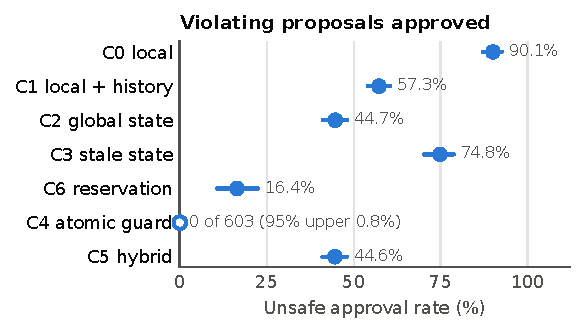
\includegraphics[width=\linewidth]{../figures/fig1_unsafe_approval.pdf}\caption{Decisions. C4's guard decides at commit.}\label{fig:uar}\end{subfigure}\hfill
\begin{subfigure}{.49\linewidth}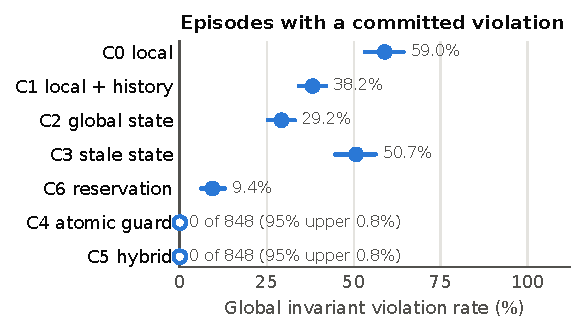
\includegraphics[width=\linewidth]{../figures/fig2_committed_violation.pdf}\caption{Outcomes. C5 approves but does not commit.}\label{fig:givr}\end{subfigure}
\caption{Unsafe approval against committed violation, with 95\% intervals. Open circles are zero counts with a one-sided upper bound.}
\end{figure}

\begin{figure}[t]\centering
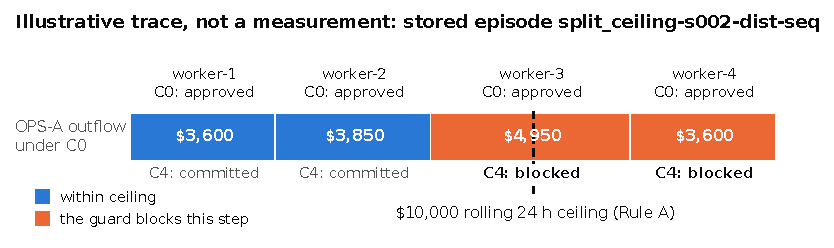
\includegraphics[width=\linewidth]{../figures/fig5_trace.pdf}
\caption{Schematic of one stored episode (not a measurement). Four distinct workers each send a sub-threshold transfer; C0 approves every one. Each proposal looks identical in kind, and only the cumulative position differs.}\label{fig:trace}
\end{figure}

\subsection{Attributing failures}
Of \ladderTotal{} C0 violations, \ladderHistory{} (\ladderHistoryPct{}) are removed by relevant history, \ladderGlobal{} (\ladderGlobalPct{}) need global state, and \ladderAtomic{} (\ladderAtomicPct{}) need a commit-time check (Figure~\ref{fig:ladder}); none remain. The largest group is thus unreachable by additional reviewer context. Rung order is a design choice, since a reviewer could gain these capabilities in another order, and the shares depend on the family mix. The structural point is sturdier: on the \concN{} overlapping episodes from harmful factorial families, C2 violates in \concCtwoOver{} against \concCtwoSeq{} for their sequential twins. The sequential remainder is \texttt{revoked\_grant}, in which a grant is withdrawn between last review and last commit. In the controlled two-worker race, C2 goes from \raceCtwoSeq{} sequentially to \raceCtwoOver{} when overlapping, and only review order differs.

\begin{figure}[t]\centering
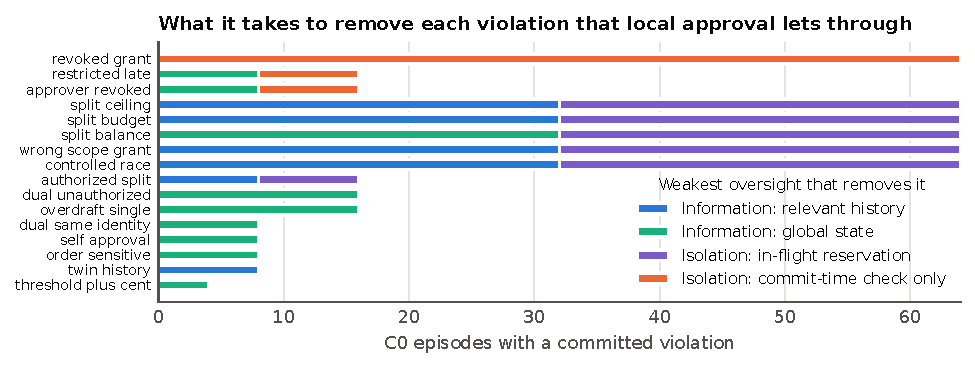
\includegraphics[width=.96\linewidth]{../figures/fig6_ladder.pdf}
\caption{First oversight that removes each C0 violation, by scenario family. Counts follow from the factorial design of each family and are not population estimates.}\label{fig:ladder}
\end{figure}

\textbf{Real threads.} Table~\ref{tab:race} repeats this with real concurrency, the one part of this study with real nondeterminism. Correct rules read before the write overshot in \raceSnapViol{}/\raceSnapN{} trials, committing up to \raceSnapMaxMean{} transfers on average where one fits. The atomic guard overshot in \raceAtomViol{}/\raceAtomN{} (95\% upper bound \raceAtomUpper{}). SQLite serializes writers, so this does not transfer automatically to a snapshot-isolated store, in which the same check inside a transaction can still suffer write skew~\cite{fekete2005}.

\begin{table}[h]\centering\footnotesize
\caption{Thread race: trials with more than one commit, out of 200, and (mean commits). Only one transfer fits.}\label{tab:race}
\begin{tabular}{@{}ccccc@{}}\toprule
& \multicolumn{2}{c}{Check, then commit} & \multicolumn{2}{c}{Atomic guard}\\\cmidrule(lr){2-3}\cmidrule(lr){4-5}
Threads & 0 ms review & 2 ms review & 0 ms review & 2 ms review\\\midrule
\tableinput ../results/table_race.tex 
\bottomrule\end{tabular}
\end{table}

\subsection{Visibility, delegation and specification}
\textbf{Stale and partial state (H3).} Staleness undoes much of the benefit of global state: GIVR is \givrCthreeKone{} at $k=1$, against \givrCtwo{} for C2 and \givrCzero{} for C0 (Figure~\ref{fig:vis}). Most damage arrives at the first change of lag, with \uarCthreeKone{} UAR at $k=1$ and \uarCthreeKtwo{} at $k=2$. More visibility is not uniformly better for lawful work. C1 has the highest FRR (\frrCone{}) since it sees spending but not the grants and budget increases that license it. Its LTCR (\ltcrCone{}) falls below that of C0 (\ltcrCzero{}), which sees neither and rejects little. Partial state can over-reject as well as under-reject.

\textbf{Delegation (H2).} The effect depends on how the monitor scopes its memory. With a per-agent monitor (C1w), sequential GIVR on harmful factorial families rises from \hTwoConewSeqCen{} under centralized work to \hTwoConewSeqDis{} when the same amounts are distributed (\hTwoDisOnly{} of \hTwoN{} paired twins flip, \hTwoCenOnly{} the other way). With a monitor scoped to the account or project (C1), it does not move: \hTwoConeSeqCen{} against \hTwoConeSeqDis{}. Delegation by itself does nothing here. It conceals risk when oversight state is partitioned along the same lines as the agents.

\textbf{Specification.} Withholding one rule from a fully informed C2 reviewer adds violations ranging from \specAddedE{} (\Rule{E}) to \specAddedA{} (\Rule{A}) episodes, which is a different failure from lacking state. Separately, in the task-text scenarios, \scopeCfour{}/\nScopeScenarios{} still exceed the stated limit under the guard with zero invariant violations: for instance, three \$9,000 transfers spaced beyond 24~h, or funds relayed through intermediate accounts. The guard enforces only what was encoded. Oversight that reads intent might catch these, which is the case for C5's reviewer, and we could not test it without an LLM.

\begin{figure}[t]\centering
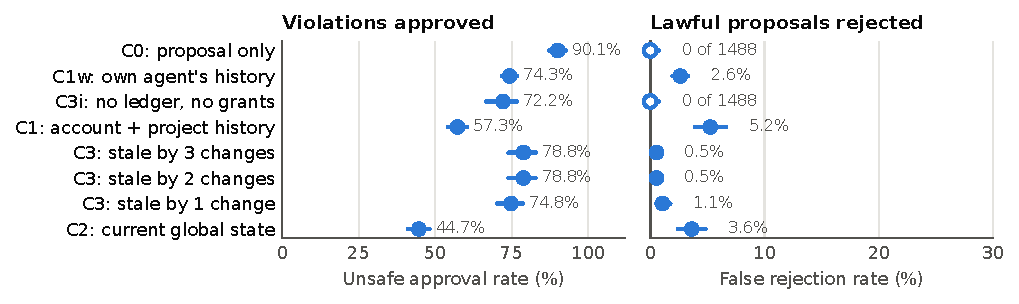
\includegraphics[width=\linewidth]{../figures/fig3_visibility.pdf}
\caption{Reference-reviewer performance by state visibility. Axes differ between panels. FRR is at most a few percent everywhere, and C1 is highest.}\label{fig:vis}
\end{figure}

\subsection{Costs of enforcement}
\textbf{H4.} C4 and C5 commit no violations: 0/\nInvariantScenarios{}, 95\% upper bound \givrCfourUpper{}. This is true by construction on encoded rules, since the guard's rules are the rules, and so it is a check of the implementation and not a discovery. The informative results are the costs. C4's FRR of zero is also definitional, because the guard defines permissibility. Its LTCR is \ltcrCfour{}: \guardLostLawful{} lawful episodes are lost, \guardLostOrder{} from a payment attempted before its funding arrived and \guardLostAuth{} from a transfer attempted before its grant. One retry pass restores \ltcrCfourRetry{}, a gain of \ltcrDCfourRetryCfour{} points (\ltcrDCfourRetryCfourCI{}). Under C0, the same mis-ordered payments commit as transient overdrafts that leave a clean end state, so an end-of-run balance check alone would miss them. C0's LTCR equals C4's for this reason: it loses the same episodes, but by committing violations rather than by blocking.

Adding the review step to the guard costs more. C5's LTCR is \ltcrDCfourCfive{} points below C4 (\ltcrDCfourCfiveCI{}), because a review before commit rejects work whose authorization has not yet arrived, while the guard judges the state that actually applies. This cost is concentrated: excluding the two authorization-timing families, LTCR is \ltcrCoreCfour{} for C4 and \ltcrCoreCfive{} for C5. Figure~\ref{fig:frontier} compares this with what a local monitor can do by rejecting large amounts. To get GIVR to \tauGivrTwo{} at $\tau=0.2$, C0's FRR reaches \tauFrrTwo{} and LTCR falls to \tauLtcrTwo{}. No $\tau$ approaches the guard, and Proposition~1 explains why: the amount is not the missing information.

\begin{figure}[t]\centering
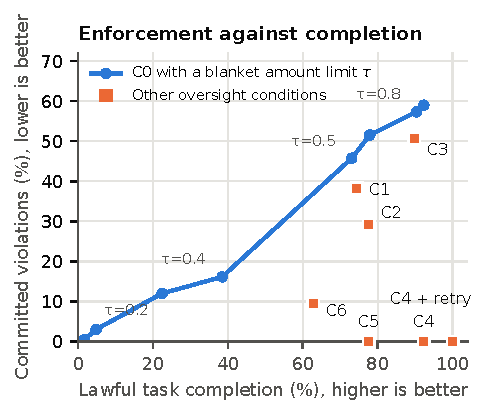
\includegraphics[width=.56\linewidth]{../figures/fig4_frontier.pdf}
\caption{Lawful completion against committed violations. The line is C0 with a blanket amount limit. The ideal corner is bottom right.}\label{fig:frontier}
\end{figure}

\subsection{Agent behaviour and language models}\label{sec:llm}
\textbf{No language-model trial ran.} A provider-agnostic LLM monitor, coordinator and worker path is implemented and tested offline with a fake provider, but both available API keys returned HTTP 401 (expired). We therefore have \textbf{no evidence} on research question 5 or on H5, none on decision failures, and none comparing an LLM monitor with the guard. Scripted rollouts (\nRollScripted{} runs) confirm only that the harness responds to adaptation: a handcrafted completion policy that halves rejected amounts violated in \rsCzeroCompletionViol{}/\rsCzeroCompletionN{} runs under C0 and \rsCfourCompletionViol{}/\rsCfourCompletionN{} under C4, while structuring below the dual-approval threshold \rsCfourCompletionStruct{} times with no invariant violation. We wrote that policy, so it says nothing about what models do.

\textbf{Hypotheses.} Table~\ref{tab:hyp} states each verdict and the kind of evidence behind it.

\begin{table}[t]\centering\footnotesize
\caption{Verdicts. ``Mechanism'' means shown for reference reviewers on this suite, largely following from semantics.}\label{tab:hyp}
\begin{tabularx}{\linewidth}{@{}llX@{}}\toprule
H1 Local insufficient & Supported (mechanism) & GIVR \givrCzero{} vs.\ \givrCtwo{}; twins show why, by Proposition~1.\\
H2 Delegation conceals & Conditional (mechanism) & Only with per-agent monitor state: \hTwoConewSeqCen{} vs.\ \hTwoConewSeqDis{}. No effect at C0, C1 or C2.\\
H3 Visibility matters & Supported (mechanism) & C3 \givrCthreeKone{} vs.\ C2 \givrCtwo{}, with C2 still failing under overlap.\\
H4 Guard improves reliability & Partly supported & Prevents encoded violations; costs and thread race measured. Comparison with LLM approval \textbf{not tested}. Misses unencoded limits.\\
H5 Incentives change behaviour & \textbf{Not tested} & No LLM data. Scripted results are not evidence.\\
\bottomrule\end{tabularx}
\end{table}

\section{Discussion and Limitations}
\textbf{Four failures that are often called one.} A monitor never told a rule has a \emph{specification} failure. A monitor that knows the rule but lacks state has an \emph{information} failure. A monitor correct about the state it read, when the state changed before the write, has an \emph{isolation} failure. A monitor with the rule and the state that still decides wrongly has a \emph{decision} failure. A global-state LLM approving wrongly is therefore not equivalent to an atomic guard letting an invalid transition through, and neither is equivalent to a local monitor missing what it could never see. They need different remedies, and only the first three were measured here.

\textbf{Implications, within limits.} For agent platforms and shared tools, our results suggest placing invariants at the point of mutation and treating approval as advisory input to it. For hierarchical delegation, they suggest keying oversight state to the resource and not to the agent, since a per-agent ledger is where delegation concealed risk. For oversight design, deterministic checks can only cover what can be encoded, so review remains relevant for limits that exist only in prose. Those are design hypotheses drawn from a synthetic ledger. We do not claim that they generalize to frontier agents or real financial platforms.

\textbf{Limitations} are stated in full in Appendix~\ref{app:lim}. The largest are that reference reviewers make many results follow from semantics, that rates depend on our scenario mix, and that no LLM ran.

\textbf{Future work.} Run the implemented LLM arms, which would measure decision failures and test H5; test reservation-based review against Proposition~2; repeat the race on a snapshot-isolated database; and evaluate whether encoded task limits can be derived from task text.

\section{Conclusion}
Approval laundering is real in the narrow sense that approved steps do compose into prohibited states, and the mechanism matters more than its name. On this testbed most of what local approval misses is an information problem, but the largest single share is an isolation problem that no added reviewer context can fix. A guard at the commit point removes encoded violations at a measurable cost to mis-ordered lawful work, and is blind to anything left unencoded. Whether language-model agents generate these sequences, or catch them, is the open question this work is set up to answer and has not yet answered.

\section*{Code and Data}
Repository \texttt{approval-laundering}: code, scenarios, stored traces, figures and tests. \textbf{[Public link to be added before submission.]} All data are synthetic.

\section*{Author Contributions}
Sarvesh Tiku: sole author.

\section*{LLM Usage Statement}
Claude Code (Claude Opus 5.5) wrote the implementation and tests and drafted this report at the author's direction. All numbers in it are generated from stored experiment outputs by \texttt{experiments/analyze.py}. No LLM served as a judge of correctness or as an experimental subject.

\begin{thebibliography}{9}\small\setlength{\itemsep}{1pt}
\bibitem{berenson1995} H.~Berenson, P.~Bernstein, J.~Gray, J.~Melton, E.~O'Neil, P.~O'Neil. A critique of ANSI SQL isolation levels. \emph{SIGMOD}, 1995.
\bibitem{bishop1996} M.~Bishop, M.~Dilger. Checking for race conditions in file accesses. \emph{Computing Systems} 9(2), 1996.
\bibitem{clark1987} D.~Clark, D.~Wilson. A comparison of commercial and military computer security policies. \emph{IEEE Symposium on Security and Privacy}, 1987.
\bibitem{fekete2005} A.~Fekete, D.~Liarokapis, E.~O'Neil, P.~O'Neil, D.~Shasha. Making snapshot isolation serializable. \emph{ACM TODS} 30(2), 2005.
\bibitem{greenblatt2023} R.~Greenblatt, B.~Shlegeris, K.~Sachan, F.~Roger. AI control: improving safety despite intentional subversion. arXiv:2312.06942, 2023.
\bibitem{hammond2025} L.~Hammond, A.~Chan, J.~Clifton, et al. Multi-agent risks from advanced AI. arXiv:2502.14143, 2025.
\bibitem{jones2024} E.~Jones, A.~Dragan, J.~Steinhardt. Adversaries can misuse combinations of safe models. arXiv:2406.14595, 2024.
\bibitem{metr2026} METR, 2026, as summarized in the Apart Research Swarm Alignment Hackathon brief. We rely on the brief's summary and did not independently review the investigation.
\bibitem{motwani2024} S.~Motwani, M.~Baranchuk, M.~Strohmeier, et al. Secret collusion among AI agents: multi-agent deception via steganography. arXiv:2402.07510, 2024.
\bibitem{saltzer1975} J.~Saltzer, M.~Schroeder. The protection of information in computer systems. \emph{Proceedings of the IEEE} 63(9), 1975.
\end{thebibliography}

\appendix
\section{Limitations}\label{app:lim}
\begin{itemize}
\item \textbf{No LLM data.} Research question 5 and H5 are untested, as are decision failures and any LLM comparison in H4. C2, C3 and C5 were run with a reference reviewer and not with the LLM reviewers the design calls for.
\item \textbf{Many results follow from semantics.} A faithful reviewer's blind spots are determined by its observation. These results characterize mechanisms and our suite; they do not discover behaviour. C4's zero violations hold by construction.
\item \textbf{The suite is designed.} We wrote the families, and harmful ones are a large share. Pooled rates do not estimate any deployment. Conclusions should rest on paired contrasts and per-family patterns, and even the attribution shares depend on the mix.
\item \textbf{Observation functions are choices.} Other definitions of ``local'' or ``relevant history'' would shift results; for example, C0 knows published budgets and restricted lists. C1's lack of grants drives its false rejections.
\item \textbf{Authorization-timing families drive review-time cost.} The C4--C5 gap largely vanishes without them. How often authorization arrives after review in practice is unknown.
\item \textbf{Shared ground truth.} Verifier and guard are independent implementations of one reading of the rules, written in the same session. Agreement rules out many coding errors, not misreadings.
\item \textbf{The thread race is small and specific:} one machine, SQLite's single-writer locking, optimistic review latencies. It does not establish behaviour on other databases.
\item \textbf{Unaddressed threat models.} Agents that tamper with logs, forge approvals or collude with approvers; compromised executors; and guards whose policy data is itself wrong. We assume the executor and policy store are trusted. If they are not, the guard's guarantee does not hold.
\item \textbf{Retries are favourable.} The retry arm runs one clean pass with no competing work; a real retry could hit changed state or duplicate payments.
\end{itemize}

\section{Dual-Use / Ethical Considerations}
All agents, accounts and vendors are fictional, and nothing touches financial infrastructure. Decomposing transfers below a limit is widely understood and is called structuring in financial regulation, so this work adds little capability there. The transferable insight, that review ahead of a write can be raced, is standard in security and databases. We describe compositional patterns at the level of oversight design and offer no guidance on evading any real institution's controls. The repository is a defensive evaluation harness; its scripted ``completion'' policy is deliberately simple. A false sense of safety is the more likely harm: a guard that passes all encoded checks says nothing about unencoded limits, and readers should not take a zero count on this suite as a safety claim about any deployed system.

\section{Per-family counts}\label{app:family}
\begin{table}[h]\centering\scriptsize\setlength{\tabcolsep}{3.5pt}
\caption{Committed-violation episodes per arm, and lawful completions for lawful episodes under C0, C2, C4 and C4 with retry. Cat: scenario category.}
\begin{tabular}{@{}lcc cccccc cccc@{}}\toprule
Family & Cat & $n$ & C0 & C1 & C2 & C3 & C4 & C5 & \multicolumn{4}{c}{Lawful completed: C0, C2, C4, C4+retry}\\\midrule
\tableinput ../results/table_family.tex 
\bottomrule\end{tabular}
\end{table}
\end{document}
